%LTeX: language=en-GB
\documentclass[a4paper,12pt]{article}

% ---------- Page setup ----------
\usepackage[a4paper,margin=2.5cm,headheight=15pt]{geometry}
\usepackage{fontspec, xcolor}
\setmainfont{LiterationSerif Nerd Font}
\setsansfont{LiterationSans Nerd Font}
\setmonofont{LiterationMono Nerd Font}[Scale=MatchLowercase]
\setlength{\parindent}{0pt}
\definecolor{codebg}{gray}{0.9}
\usepackage[british]{babel}
\emergencystretch 1.5em

% ---------- Useful packages ----------
\usepackage{microtype}
\usepackage{float}
\usepackage{graphicx}
\graphicspath{{./images/}}
\usepackage{tabularx}
\usepackage{caption}
\usepackage{subcaption}
\usepackage{makecell}
\renewcommand{\theadfont}{\bfseries\normalsize}
\usepackage{amsmath,amssymb}
\usepackage{upquote}
\usepackage{fancyhdr}
\usepackage{setspace}
\usepackage{minted}
\setminted{fontsize=\normalsize, baselinestretch=1, bgcolor=codebg}
\usepackage{hyperref}
\usepackage{citation-style-language}
\usepackage{xltabular}
\usepackage{booktabs}
%\cslsetup{style = ieee-wrexham_v7}
%\addbibresource{references.bib}

% ---------- Custom commands -------------
\makeatletter
\newcommand\code{%
  \begingroup
  \catcode`\_=12 \catcode`\$=12 \catcode`\#=12
  \catcode`\%=12 \catcode`\&=12 \catcode`\^=12
  \code@i
}
\newcommand\code@i[1]{%
  \endgroup
  \setlength{\fboxsep}{0.5pt}%
  \mbox{\colorbox{codebg}{\normalsize\texttt{#1}}}%
}
\makeatother

% ---------- Document variables ----------
\newcommand{\myname}{Christoph Schabik, Sven Ziegler, Maximilian Leidl, Alina Pollich}
\newcommand{\mystudentid}{S26007467, S26008938, S26010157, S26008939}
\newcommand{\mytitle}{Assignment}
\newcommand{\mycourse}{Systems Engineering and Project Management / COM569}
\newcommand{\mysupervisor}{Daren Morris, Jose Bindu}
\newcommand{\myuniversity}{Wrexham University}
\newcommand{\myfaculty}{Cyber and Computing}

% ---------- Header/Footer ----------
\pagestyle{fancy}
\fancyhf{}
\rhead{\thepage}
\lhead{\leftmark}
\renewcommand{\headrulewidth}{0.4pt}

\onehalfspacing

% ---------- Title page info ----------
\title{\mytitle}
\author{\myname \\ Student ID: \mystudentid}
\date{\today}

\begin{document}

% ---------- Title Page ----------
\begin{titlepage}
	\centering
	\vspace*{2cm}
	{\Large \myuniversity\par}
	\vspace{0.5cm}
	{\large \myfaculty\par}
	\vspace{2cm}
	{\Huge\bfseries \mytitle\par}
	\vspace{1.5cm}
	{\large \mycourse\par}
	\vspace{2cm}
	{\large \textbf{Author:} \myname\par}
	{\large \textbf{Student IDs:} \mystudentid\par}
	{\large \textbf{Supervisors:} \mysupervisor\par}
	\vfill
	{\large \today\par}
\end{titlepage}

\tableofcontents
\listoffigures
\listoftables
\newpage

% ---------- Content ----------
\section{Introduction}

\section{Project Charter}
\subsection{Scope}
This Project aims to create the MVP (Minimal Valuable Product) of CodeBrew, which includes the features \textbf{company registration}, \textbf{company login}, \textbf{form creation}, \textbf{display of statistics}, \textbf{customer can fill out the form} and the \textbf{voucher generation}.
Consequently, are all resources included, which are needed to archive the functionality of these features (database, REST-API, webpage, ...).
This MLP is also described by the following use case diagram \autoref{fig:use_case}.

\begin{figure}[H]
	\centering
	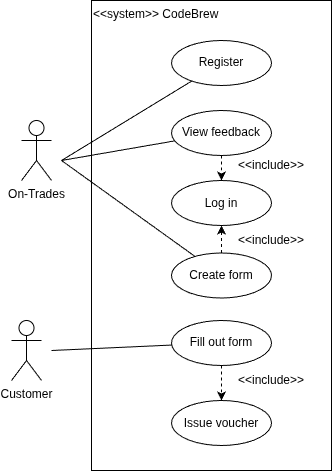
\includegraphics[width=0.5\textwidth]{use_case.drawio.png}
	\caption{Use case diagram}
	\label{fig:use_case}

\end{figure}

\subsection{Constraints}
The form which can be created by a company is at the start just a \textbf{static template} where the different beers, which the on-trade company sells, can be selected.
Which beers are selectable is also static. Beers can only be added by the CodeBrew team.

\subsection{Initial resources}
The project's human resources are 2 backend developer, 1 database engineer, 1 frontend developer, which is additionally the project owner.
Every developer has access to one personal computer on which they will develop.
GitHub was chosen as centralised git provider and kanban host (GitHub Project).

\subsection{Authority of the project manager}
The project management is part of the job of the project owner. The project manager will be supported by the project team.
Every decision in terms of feature changes or time extensions  has to be approved by the project owner.
Tasks on the kanbanboard are created by the project manager collaborative with the project team.
The team is not allowed to create tasks without the knowledge of the project owner.

\section{Stakeholders}
\subsection{Stakeholder Identification}
Identifying stakeholders during the planning phase is essential to ensure that their requirements can be addressed in subsequent phases.

\subsubsection{Primary Stakeholders}
The following groups are identified as primary stakeholders as they are directly involved in the development or operation of the system.

\begin{itemize}
    \item \textbf{On-Trade Companies} are interested in customer feedback to optimise their beverage offering and attract new customers through vouchers.
    They have a high influence on the application, as they represent the primary customers to whom the system is marketed. 
    They should be involved in the development process to ensure their requirements are met.
    \item \textbf{Bar patrons} are interested in a fast and straightforward feedback process. 
    They have a high influence on the development, as the system will not be used if the process is flawed or overly complicated.
    \item The \textbf{CodeBrew Development Team} is interested in meeting all requirements, establishing a clean system architecture, and developing a functional system. 
    Meeting existing deadlines is also a key objective. They have a very high influence as they are responsible for managing scope, design, security, and technical implementation.
    \item The \textbf{University Staff (Product Sponsor)} is interested in ensuring that students learn and adhere to systems engineering and project management methodologies. 
    Furthermore, the goal is to produce a viable product with added value from the planning phase onward, while implementing a robust and secure system architecture. 
    They have a very high influence on the project, as they define the specifications and acceptance criteria and perform the final evaluation of the project. 
    They must be integrated into the development process.
\end{itemize}

\subsubsection{Secondary Stakeholders}
Parties that are only indirectly affected or involved in regulation must also be identified as secondary stakeholders.

\begin{itemize}
    \item \textbf{Legislators and Authorities} are interested in ensuring that personal data is processed lawfully and that regulations regarding youth protection are upheld. 
    They have a high influence on the project, as it is crucial to ensure that legal requirements are met. Non-compliance can lead to severe legal consequences.
    \item \textbf{Beverage Suppliers} are interested in knowing which varieties are most in demand. 
    They currently have very low influence on the project, as they are not directly involved in the feedback process at this stage.
\end{itemize}

\subsection{Engagement Strategy}
The engagement strategy serves to determine how and how often the respective stakeholders are involved in the project's progression to ensure its success. 
To this end, the identified stakeholders are categorised into the groups \textit{Manage Closely}, \textit{Keep Satisfied}, and \textit{Monitor}.

\subsubsection{Manage Closely}
These stakeholders have both high influence and high interest. They are critical to the success of the project and are actively involved in the development process.

\begin{itemize}
    \item \textbf{On-Trade Companies} will be involved early in the development process to meet customer expectations. 
    For instance, operators can be consulted on designs for the dashboard and specific functions.
    \item The \textbf{CodeBrew Development Team} must ensure continuous information exchange and good self-organisation. 
    This is achieved through regular meetings with logbook documentation, task distribution via Kanban, and a clear distribution of roles.
    \item The \textbf{Product Sponsor} must be included in the acceptance process through regular gate reviews and access to the project progress documentation.
\end{itemize}

\subsubsection{Keep Satisfied}
These stakeholders are relevant to the project but have a more passive interest and are therefore not actively involved in the development process.

\begin{itemize}
    \item To provide \textbf{Bar patrons} with a pleasant user experience, the focus will be on a simple and intuitive user interface.
    Additionally, the entire feedback process and subsequent rewards will be designed to be as uncomplicated as possible.
    \item The requirements of \textbf{Legislators and Authorities} must be met through strict adherence to guidelines.
    This can be ensured through age verification and the appropriate handling of personal data.
\end{itemize}

\subsubsection{Monitor}
These stakeholders have low relevance at the current stage of the project. However, they should not be ignored, as they may become more important in the future.

\begin{itemize}
    \item \textbf{Beverage Suppliers} are not currently involved in the feedback process. 
    They could, however, be integrated in the future, and market analyses could be provided to them. 
    To facilitate this, the database architecture must be cleanly structured from the outset.
\end{itemize}


\subsection{Stakeholder Requirements}
Following the identification of the stakeholders and the definition of the engagement strategy, 
the specific requirements of the stakeholders are identified. 
These are fundamental for identifying the system requirements and to ensure that the needs of the stakeholders are met. 
The following Table \ref{tab:stakeholder_requirements} lists the corresponding requirements.
{
\renewcommand{\arraystretch}{1.7}
\begin{xltabular}{\textwidth}{c p{2.5cm} p{4cm} X}

\caption{Stakeholder Requirements}
\label{tab:stakeholder_requirements} \\
\toprule
\textbf{No.} & \textbf{Stakeholder} & \textbf{Need} & \textbf{Requirement} \\ 
\midrule
\endfirsthead

\caption{Stakeholder Requirements (Continued)} \\
\toprule
\textbf{No.} & \textbf{Stakeholder} & \textbf{Need} & \textbf{Requirement} \\ 
\midrule
\endhead

\bottomrule
\endfoot

1 & On-Trade Companies & The operator requires their specific beer assortment to be available for customer feedback. & 
The system must provide a pre-configured, specific list of beer types in the feedback form based on prior arrangement. \\
2 & On-Trade Companies & The operator requires a way to evaluate feedback. & 
The system must aggregate collected customer reviews per beer type and present them graphically to the operator. \\
3 & On-Trade Companies & There must be protection against voucher misuse. & 
The system must prevent multiple redemptions of vouchers by the same guest at the same location through blocking mechanisms. \\
4 & Bar patrons & Guests require intuitive access to the application. & 
The system must allow guests to open the feedback form directly via a QR code scan without prior registration. \\
5 & Bar patrons & Guests should receive their rewards in a straightforward manner. & 
The system must generate the voucher immediately after the feedback is submitted. \\
6 & Bar patrons & An efficient rating system is required. & The system must allow guests to rate multiple beer types within a single session. \\
7 & CodeBrew Development Team & A clean system architecture should be established. & 
The system must feature a clear separation between frontend and backend, a normalised database design, and well-structured interfaces. \\
8 & CodeBrew Development Team & Seamless and transparent collaboration is required. & 
The project must be based on standardised workflows, including a unified development environment, version control strategy, and agile task tracking. \\
9 & University Staff (Product Sponsor) & Evidence of the methods used in planning and development is required. & 
The project must be documented without gaps through artefacts such as logs and UML diagrams. \\
10 & University Staff (Product Sponsor) & A functional product is required for final evaluation. & 
The system must be available as a working product at the end of the project, providing the promised features. \\
11 & Legislators and Authorities & Youth protection regulations must be complied with. & 
The system must implement an age verification check before the form can be accessed. \\
12 & Legislators and Authorities & The system must be designed to be GDPR compliant. & 
Appropriate data handling must be ensured through robust measures. \\
13 & Beverage Suppliers & The system must be prepared for future market analyses. & 
The database must be proactively structured so that aggregated exports regarding the popularity of various types can be generated in the future. \\
\end{xltabular}
}

\end{document}

\begingroup
\setstretch{1.0}
\hbadness=9999
\printbibliography
\endgroup

\end{document}
